%
%You can keep the 12pt font size, or go to 11pt or (default) 10pt
% Do NOT go any larger than 12pt font size for submission
%
%If you want to edit a printed copy, you may want to add draft mode
% (as in \documentclass[draft,conference,12pt]{IEEEtran})
% This adds space between the lines providing easier editing markup
%
%For more details see 
% http://ras.papercept.net/conferences/support/files/IEEEtran_HOWTO.pdf
%
\documentclass[conference,12pt, ]{IEEEtran}
\usepackage[margin=1truein]{geometry}
\usepackage{cite}
\usepackage{graphicx}
\usepackage{algorithmic}
\usepackage{url}
\usepackage{flushend}
\usepackage{listings}

% correct bad hyphenation here
\hyphenation{op-tical net-works semi-conduc-tor}

\begin{document}


\title{Avoiding General Purpose Microcontrollers For Multirotor Autonomous Flight }

\author{
	\IEEEauthorblockN{Innocent Niyibizi}
  \IEEEauthorblockA{Computer Science Department\\Missouri University of Science and Technology\\Rolla, MO 65409\\
  Email: iniyibizi@mst.edu}
}


% make the title area
\maketitle

\begin{abstract}
As the world continues to develop, more and more problems arise that can be solved with the use of advanced software systems. These problems can be things such as navigating an unfamiliar environment or surveying known environments after disaster strikes. To accomplish these goals, months of R\&D is poured into specific problems and how to solve them with the current technological advances. 
\end{abstract}

\section{Introduction}
Technological advances happen all throughout the country and in many different disciplines. The one that is the most notable is "drone" technology. The technology spans from tiny, harmless pocket drones to the stealthy, yet deadly, USA Military Unmanned Aerial Vehicles. With the development of drone hardware and software, we're now able to move from human operated flights into flights that are all in the control of the vehicles. The ability to have these vehicles operate without human intervention will open a number of doors for modern problems to be solved with modern solutions. This is where organizations, such as The International Aerial Robotics Comptetition (IARC), comes into play.\\
The IARC is an competition that strives to push the boundaries of aerial flights and problem solving. Each year year they have so called missions for what they consider to be the most important area of focus. These missions can range from autonomously flying around a given area to autonomously herding Roomba vacuum cleaners in a 25mx25m gym onto one side. Each mission will have its fair share of restrictions and technological advances that must be had before the mission can be completed. \\
These missions are geared towards college teams/organizations to take their shot solving the issue which opens the door for creative. A design team on campus, The Multirotor Robot Design Team(MRR) is one such team and has been tackling this since 2016. They have gone through many microcontrollers, specifically flight boards, and have found the feasibility of each one for the given task.

\section{History}
MRR has been in the autonomous flight field since the very beginning but they could not have gotten there without the short comings and the lessons learned along the way. One of the most important things learned along the way, is the need for the right sensors and flight board for autonomous based tasks. The team experimented with two microcontrollers before settling with one that really suites their needs. Each one has its unique features and feasibility to the challenge at hand: Fly autonomously in an indoor environment with limited sensor input. 

\subsection{APM Flight Board}
This is where discussions for APM will take place.

\subsection{Arduino}
This is where the Arduino will come into play.

\subsection{Pixhawk}
This is where the Pixhawk will be torn apart, smh it needs to be stopped. 

\section{The Microcontrollers That Could}
\subsection{APM Flight Board: Captain}
\begin{figure}
	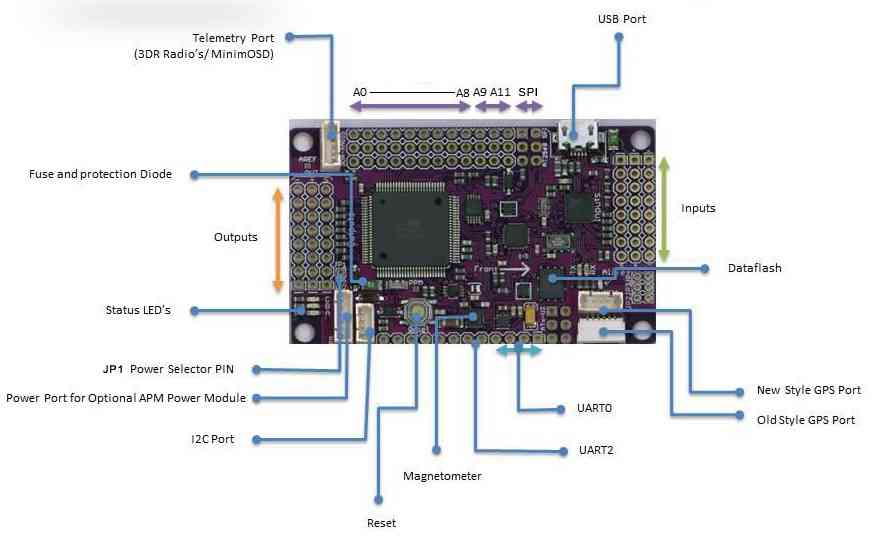
\includegraphics[scale=0.40]{apm2.jpg}
	\caption {Layout of APM2.5 Flight Controller}
\end{figure}
\subsubsection{Features}
Talk about the features
\subsubsection{Use Cases}
Talk about the many use cases
\subsubsection{Task Feasibility}
Talk about if the task is even possible given the steaks.


\subsection{Arduino: Mega}
\begin{figure}
	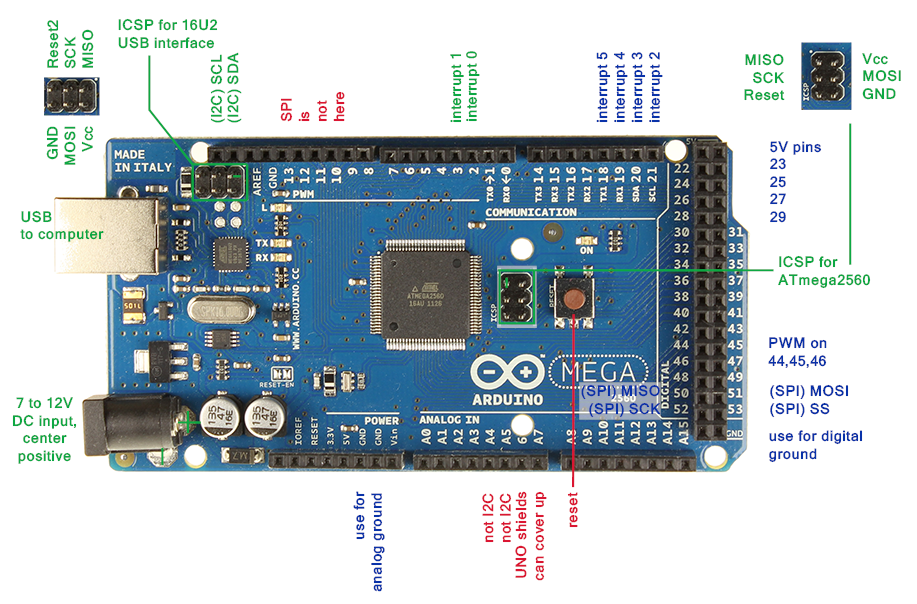
\includegraphics[scale=0.25]{mega.png}
	\caption {Layout of Arduino Mega  Microcontroller}
\end{figure}
\subsubsection{Features}
Talk about the features
\subsubsection{Use Cases}
Talk about the many use cases
\subsubsection{Task Feasibility}
Talk about if the task is even possible given the steaks.

\subsection{Cortex-M4: PixHawk 2 (The Cube)}
\begin{figure}
	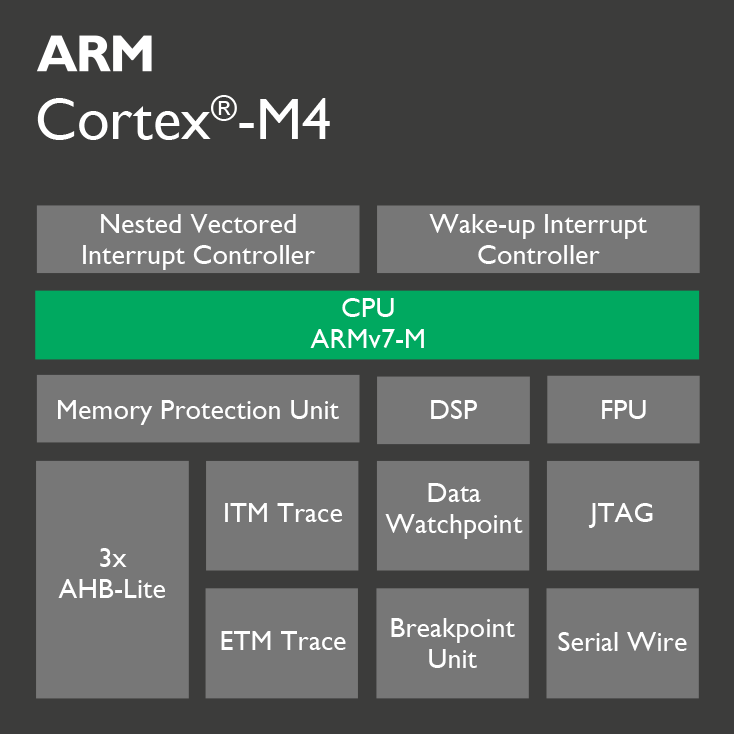
\includegraphics[scale=0.12]{cortex.png}
	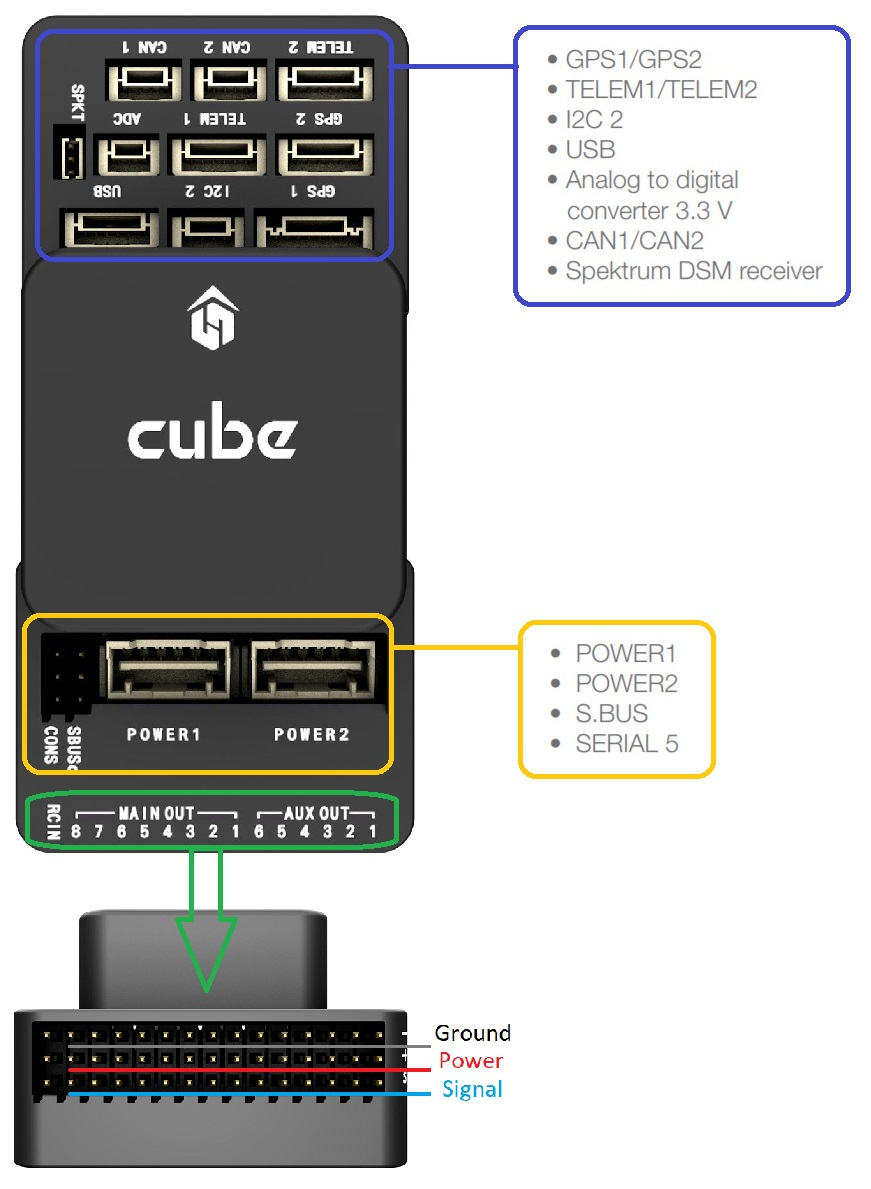
\includegraphics[scale=0.25]{cube.jpg}
	\caption{Cortex-M4 and Pixhawk 2(The Cube)}
\end{figure}
\subsubsection{Features}
Talk about the features
\subsubsection{Use Cases}
Talk about the many use cases
\subsubsection{Task Feasibility}
Talk about if the task is even possible given the steaks.



\section{Conclusion}
This section is where the paper will end and everything will make sense once again

  \begin{thebibliography}{999}

  \bibitem{linux_source} Bootlin {\em Linux source code: (v4.18.15) - Bootlin. [Online]. Available: \url{https://elixir.bootlin.com/linux/v2.6.36/source/kernel/sched.c}} [Accessed: 07-Dec-2018].

  \bibitem{virtual_runtime}  CFS Scheduler {\em [Online]. Available: \url{https://www.kernel.org/doc/Documentation/scheduler/sched-design-CFS.txt}} [Accessed: 07-Dec-2018].

  \bibitem{testing_sched} L. Jelenković, S. Groš, and D. Jakobović {\em Testing task schedulers on Linux system.} 

  \bibitem{red_black_tree} J. Morris {\em “Red Black Trees,” Data Structures and Algorithms: Hash Tables. [Online]. Available: \url{https://www.cs.auckland.ac.nz/software/AlgAnim/red_black.html}.} [Accessed: 07-Dec-2018]

  \end{thebibliography}
\end{document}

